% !TeX root = ../mat_mod2.tex

\section{\protect\raggedright
  Разработка методов учета динамических ограничений
  в~оптимизационных алгоритмах
  маршрутизации инструмента машин
  для термической резки листовых заготовок
}
\label{sect:2.3}
\setcounter{equation}{0}

Как отмечалось в \ref{sect:1.3}
наиболее сложной проблемой при разработке методов оптимизации
траектории инструмента машин листовой резки с ЧПУ
является математическая формализация и
разработка вычислительных алгоритмов учета
технологических эвристических требований термической резки,
т. н. правил <<жесткости детали>>
и <<жесткости листа>>.
<<Динамический>> характер этих условий, заключающийся в том,
что сами ограничения формируются только в процессе вычисления
допустимого решения задачи, по сути порождает
новый не исследованный ранее класс маршрутных задач
с крайне сложными видами ограничений типа
(\ref{pierce-constraint}).

Ниже приведен способ формализациии правила <<жесткости детали>>,
основанный на введении понятия <<зона жесткости>>.

\begin{opred}
  {\bf Зоной жесткости}
  называется область,
  ограниченная следующими четырьмя геометрическими кривыми:
  1) траекторией инструмента;
  2) эквидистантной этой траектории кривой, отстоящей на величину $R$;
  3) прямой, проходящей через точку выключения инструмента $M^*$
  перпендикулярно траектории инструмента в этой точке;
  4) прямой, проходящей через точку,
  отстоящую от точки выключения инструмента $M^*$ на некоторую величину $L$,
  перпендикулярно траектории инструмента в этой точке.
\end{opred}

Параметры этой зоны для двух точек
(длина $L$ и радиус $R$)
определяются в каждом конкретном случае
на основании экспертной оценки,
зависящей, в частности, от марки и толщины материала,
а также технологии термической резки.
На~рис.~\ref{hardness-area}
эти зоны выделены желтым цветом.

\begin{figure}[h]
 \begin{center}
  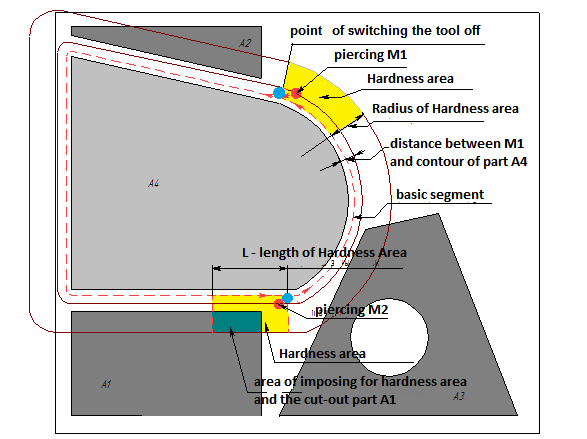
\includegraphics[width=0.9\textwidth]{hardness-area.png}
  \caption{
    Формализация правила <<жесткости детали>>
    на основе понятия
    <<зоны~жесткости>>
    }
  \label{hardness-area}
  \end{center}
\end{figure}

Тогда в оптимизационных процедурах машрутизации
для задачи GTSP  и дискретных моделей задач {\it CCP, SCCP, GSCCP}
выбор точки врезки $M$
и точки выключения инструмента $M^*$
(сегмента резки) определяется простым условием:
{\bf зона жесткости} должна лежать в еще невырезанной
<<жесткой>> части листового материала.
Для тех точек врезки, для которых это условие не выполнено,
значение целевых функций  увеличивается на некоторую величину
<<штрафа>>.

Как нетрудно видеть,
сформулированное правило выбора <<хороших>> точек врезки
и точек выключения инструмента носит геометрический характер.
Поскольку технологическое правило <<жесткости>> детали
связано с тепловыми деформациями материала,
то естественно предположить,
что температура в <<хороших>> зонах <<жесткости>> будет меньше,
чем в <<плохих>>.
В случае справедливости этой гипотезы,
адекватная оценка тепловых деформаций материала
при термической резке заготовок на машинах с ЧПУ
может иметь важное значение как инструмент
обеспечения необходимых технологических требований.
Для проверки гипотезы необходимо иметь инструментарий
моделирования и вычисления температуры тепловых полей в
каждый момент времени процесса резки.
Для разработки необходимого программного
обеспечения рассмотрим следующую задачу.

{\bf Постановка задачи}

Имеется металлическая пластина.
Заданы контуры, последовательность их резки,
точки врезки и направления обходов.
Для режущего инструмента заданы радиус теплового луча,
мощность, скорость перемещения и скорость холостого хода.
Требуется рассчитать тепловые поля при
последовательной резке контуров.

{\bf Расчет процесса резки контуров}

Последовательно для каждого контура рассматривается задача нахождения
$\theta(t, x)$ -- температуры
($t$ -- момент времени,
$x$ -- точка области),
удовлетворяющей уравнению теплопроводности
\begin{equation}
  c \rho \frac{\partial \theta}{\partial t}=k \Delta \theta +N, x \in \Omega
  ;
\end{equation}
начальному условию
\begin{equation}
  \theta(t_0, x)=\theta_0(x), x \in \Omega
  ;
\end{equation}
граничному условию
\begin{equation}
  -k \frac{\partial \theta}{\partial n}=M(\theta - \theta_*), x \in \partial \Omega
  .
\end{equation}
$t$ из промежутка $[t_0, t_1]$,
$x$ -- точка области
$\Omega \subset \mathbb R^3$.

Здесь
$t_0$ -- время начала и
$t_1$ -- время окончания резки текущего контура;
$\Omega$ -- часть пластины, которая осталась после удаления областей;
ограниченных предыдущими контурами,
$\partial \Omega$ -- граница области $\Omega$;
$c$ -- удельная массовая теплоемкость,
$\rho$ -- плотность,
$k$ -- коэффициент теплопроводности,
$N(t,x)$ -- плотность тепловых источников,
$M$ -- коэффициент теплопередачи,
$\theta_0(x)$ -- текущее температурное поле перед началом резки данного контура,
$\theta_*$ -- температура воздуха.

Функция $N$ плотности тепловых источников имеет следующий вид.
Пусть толщина листа  $h$,
радиус теплового луча $r$,
его мощность w и скорость перемещения $v$.
Пусть  $m(t)$ -- положение оси теплового луча
в момент $t$.
Тогда
$p=w/(\pi r^2 h)$
есть
плотность мощности теплового <<луча>> и
$N(t,x)=p$
в точках, находящихся от прямой $m(t)$
на расстоянии меньше $r$  и
$0$ в остальных точках.

{\bf Аппроксимация задачи}

Процесс пересчета температурного поля
$\theta(t, x)$
во время резки контура
разбивается на малые промежутки времени
$[t_{r-1}, t_r]$
длины  $\Delta t$
и для расчета
$\theta(x)=\theta(t_r, x)$
рассматривается задача
\begin{equation}
c \rho \frac{\theta(x)-\theta_0(x)}{\Delta t}=k \Delta \theta(x) + N(X)
\end{equation}
\begin{equation}
  -k \frac{\partial \theta}{\partial n}=M(\theta - \theta_*)
\end{equation}
где
$\theta_0=\theta(t_{r-1}, x)$
и
$N(x)=N(t_{r-1},x)$.

Область
$\Omega$
разбивается на тетраэдры,
функции
$\theta(x), \theta_0(x), N(x)$ -- кусочно-линейные,
определяемые значениями в узлах -- вершинах тетраэдров.
Решением задачи является точка минимума следующего функционала:
\begin{multline}
  I(\theta) =
  \frac{1}{2 \Delta t} \int\displaylimits_\Omega c \rho (\theta - \theta_0)^2 dx
  + \frac12 \int\displaylimits_\Omega k |\nabla \theta|^2 dx \\
  - \int\displaylimits_\Omega N \theta dx
  + \frac12 \int\displaylimits_{\partial \Omega} M(\theta - \theta_*)^2 dS
  .
\end{multline}

Нахождение точки минимума данного квадратичного фунционала
проводится методом релаксации.
Выбор метода основан на следующих соображениях.

Так как радиус  $r$
теплового луча мал,
то тетраэдры разбиения области должны иметь малый размер
(в расчетах длина сторона была  2 мм)
и поэтому их много.
В~узлах, далеких от точек,
где уже был тепловой луч
и куда еще не могло дойти изменение тепла к данному моменту времени,
температура остается первоначальной.
Метод релаксации позволяет пропустить такие узлы
и тем самым уменьшить время счета.

{\bf Замечание}.
Для уменьшения числа тетраэдров (узлов)
при расчете резки очередного контура
$K_i$
рассматривается не вся оставшаяся пластина, а кусок
$\Omega_i \supset \Omega_{i-1}$.
Кусок  достаточно большой,
чтобы к моменту завершения резки контура
$K_i$
температура вне
$\Omega_i$
не могла измениться.
После завершения резки контура
тетраэдры внутри контура удаляются и их число уменьшается.
Дальше производится расширение СКЭ до следующего куска
$\Omega_{i+1}$.

{\bf Просмотр результатов}

Разработанное программное обеспечение
позволяет просматривать изменение температурных полей
в процессе резки.
На~рис.~\ref{thermal-plan}
показан пример задания порядка резки
шести заготовок (восемь контуров),
точек врезки и направление обхода
(минус означает обход по часовой стрелке).
Материал пластины -- сталь 12Х2Н4А,
толщина $h$ = 2 мм,
размеры 1000 $\times$ 1000 мм.
Радиус теплового луча $r$ = 2 мм,
мощность $w$ = 1000 Вт,
скорость $v$ = 10 м/с.

На рис.~\ref{thermal-5} показано температурное поле
на одной из стадий процесса резки пятого контура.

{\bf Замечание}.
Рис. \ref{thrm-high} и~\ref{thrm-low}
иллюстрирую справедливость гипотезы.
Эти процессы отличаются только выбором точки врезки.
На рис.~\ref{thrm-high}
точка врезки вблизи кромки пластины.
Средняя температура в выделенном окне
вокруг точки завершения резки контура 480 $^\circ$С.
На рис.~\ref{thrm-low} точка врезки далеко от кромки.
Средняя температура в выделенном окне  362 $^\circ$С.

\begin{figure}
  \centering
  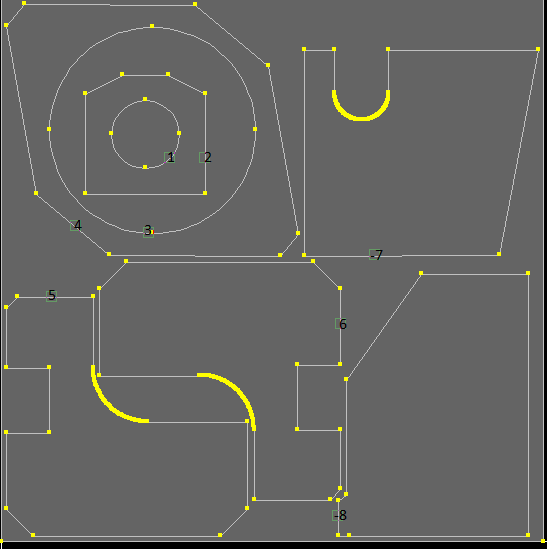
\includegraphics[width=0.6\textwidth]{thermal-plan.png}
  \caption{Места точек врезки и порядок резки для восьми контуров}
  \label{thermal-plan}
\end{figure}

\begin{figure}
  \centering
  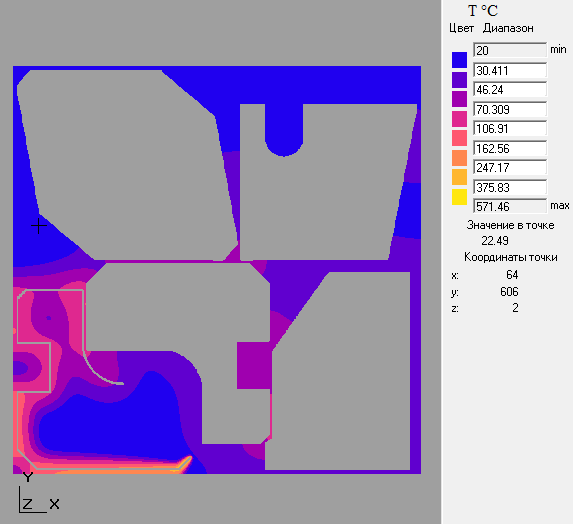
\includegraphics[width=0.7\textwidth]{thermal-5.png}
  \caption{Пример распределения тепловых полей в процессе резки пятого контура}
  \label{thermal-5}
\end{figure}

\begin{figure}
  \centering
  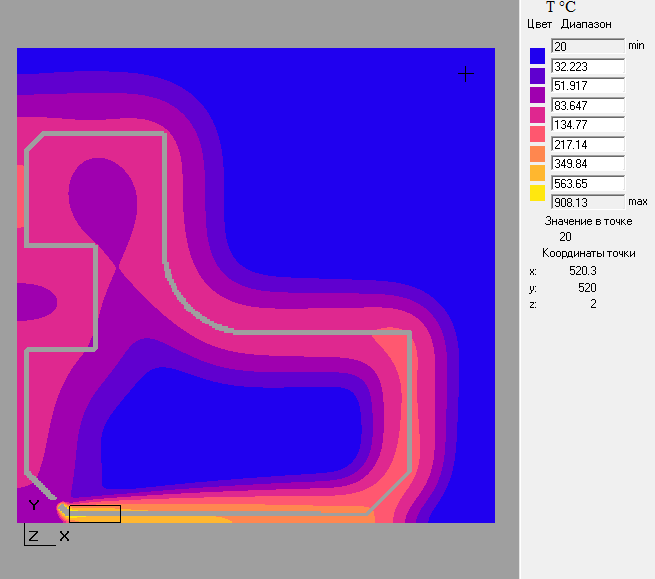
\includegraphics[width=0.6\textwidth]{thermal-high.png}
  \caption{Температурное поле при выборе точки врезки вблизи края пластины}
  \label{thrm-high}
\end{figure}

\begin{figure}
  \centering
  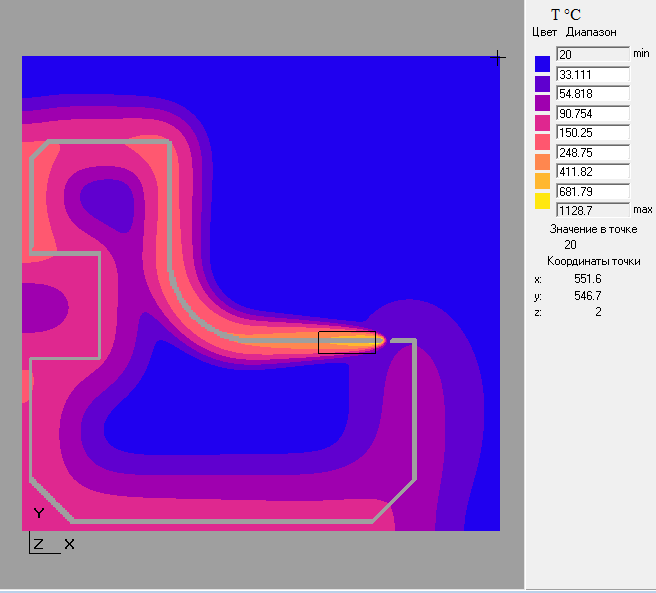
\includegraphics[width=0.6\textwidth]{thermal-low.png}
  \caption{Температурное поле при выборе точки врезки вдали от края пластины и~границ вырезанных заготовок}
  \label{thrm-low}
\end{figure}

Другие проведенные вычислительные эксперименты
также показали уменьшение температуры материала
в <<хороших>> зонах в среднем на 63 \%.
Ниже приведены еще два примера расчета температурных полей
(с нарушением правил жесткости на рис.~\ref{thermal-309}
и рис.~\ref{thermal-550}
и их соблюдением на рис.~\ref{thermal-120}
и рис.~\ref{thermal-130}).

\begin{figure}
  \centering
  \subfigure[309 $^\circ$C (точка выключения инструмента не удовлетворят правилу <<жесткости детали>>) ]{
    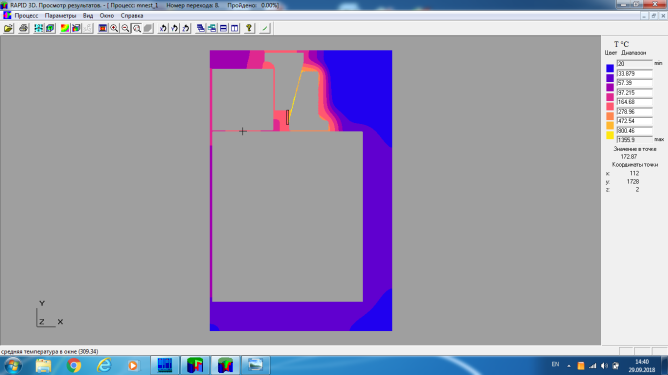
\includegraphics[width=0.9\textwidth]{thermal-309.png}
    \label{thermal-309}
  }
  \subfigure[120 $^\circ$C (точка выключения удовлетворят данному правилу)]{
    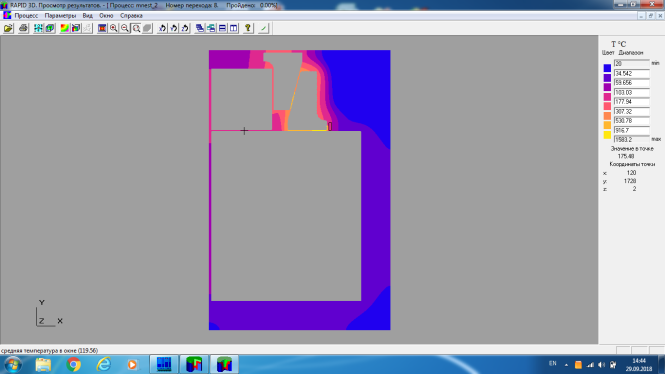
\includegraphics[width=0.9\textwidth]{thermal-120.png}
    \label{thermal-120}
  }
  \caption{Уменьшение температуры металла в зоне жесткости }
  \label{thermal-309-120}
\end{figure}

Таким образом,
анализ температурных полей подтверждает
геометрические правила выбора точек врезки
и точек выключения инструмента машин термической
резки материала и в будущем
(при условии разработки быстродействующих систем температурного анализа)
может сам служить средством для выбора точек начала и конца сегментов резки.

\begin{figure}
  \centering
  \subfigure[550 $^\circ$C]{
    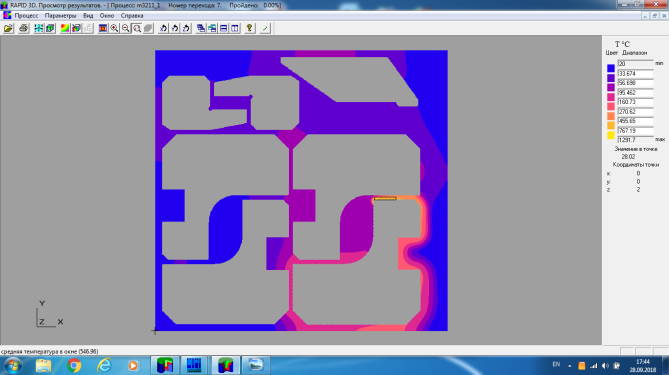
\includegraphics[width=0.9\textwidth]{thermal-550.png}
    \label{thermal-550}
  }
  \subfigure[130 $^\circ$C]{
    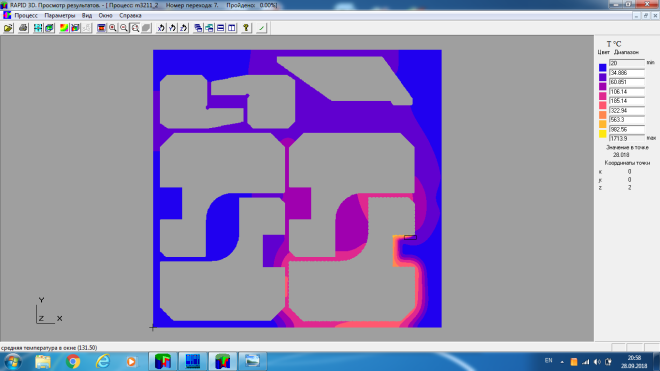
\includegraphics[width=0.9\textwidth]{thermal-130.png}
    \label{thermal-130}
  }
  \caption{Уменьшение температуры металла в зоне жесткости }
  \label{thermal-550-130}
\end{figure}

Рассмотрим далее один из простых способ учета правила жесткости листа,
описанного в \ref{sect:1.3},
основанный на делении области листа на
последовательный набор подобластей (зон):
$$
  B_j =
  \bigcup_{r=1}^l \Omega_r
  .
$$

Способ заключается в том,
что после определения направления вырезки деталей на листе
(например, слева направо),
область листа разбивается вертикальными линиями
на прямоугольники одинакового размера.
Количество прямоугольников $l$
варьируется от 4 до 10 в зависимости от
геометрических размеров деталей
(чем крупнее размеры прямоугольников,
тем меньше формируется число зон).
Затем в каждой зоне решается основная задача
(\ref{problem-statement})
уже без учета требований жесткости листа,
но с учетом правила <<жесткости детали>>
с помощью  алгоритма, описанного выше в этом параграфе.

На рис.~\ref{zones-a}
приведен пример оптимизации траектории
инструмента для задачи $GTSP$ с учетом
формирования подобластей.
Число подобластей в данном примере -- пять.

\begin{figure}
  \begin{center}
  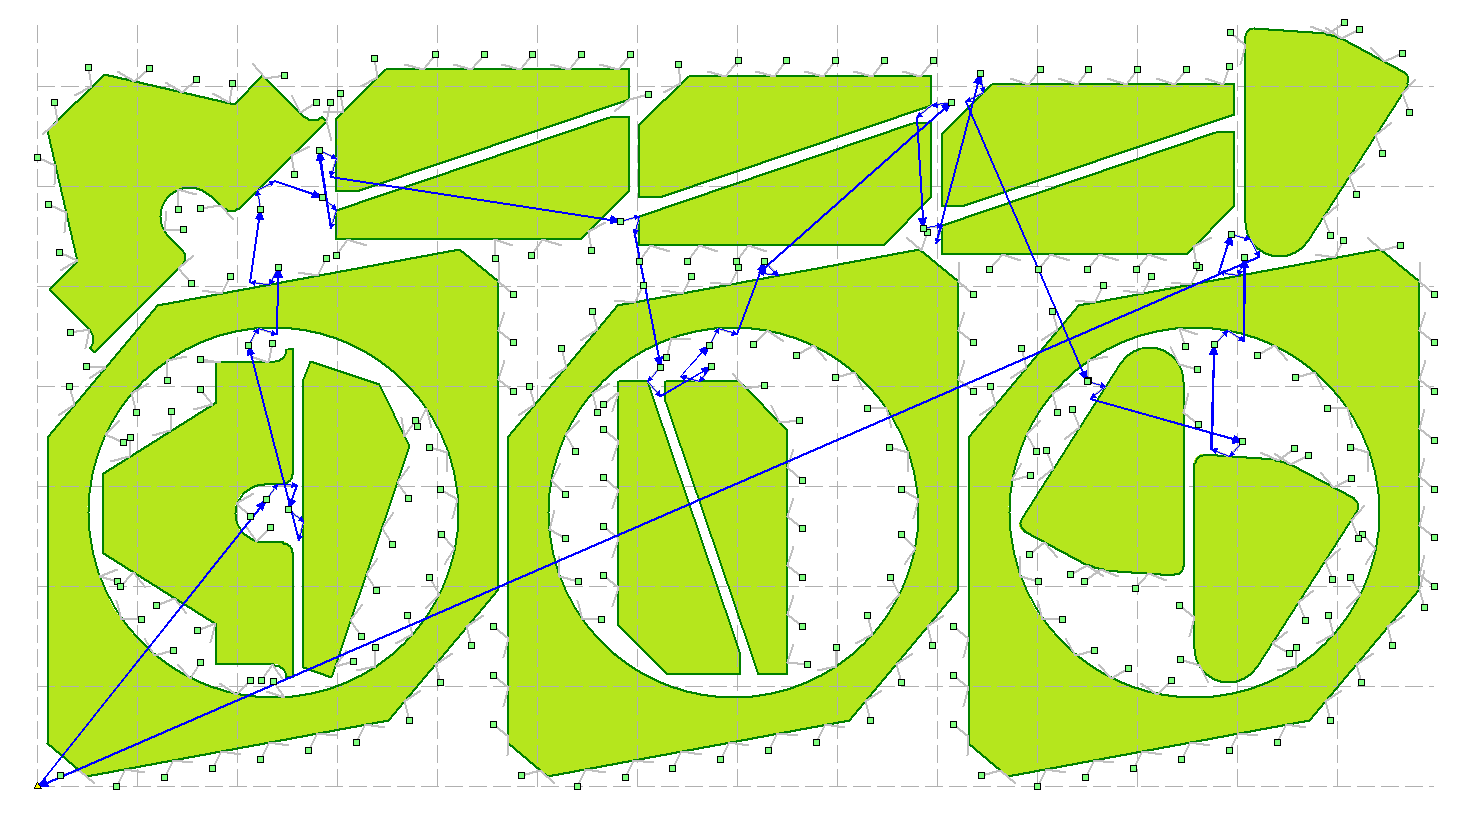
\includegraphics[width=0.9\textwidth]{zones-a.png}
  \caption{
    Пример моделирования траектории инструмента машины листовой резки с~ЧПУ
    с~учетом правила <<жесткости листа>>
    и~с~использованием зон
    (20~контуров, задача $GTSP$)
    }
  \label{zones-a}
  \end{center}
\end{figure}

На рис.~\ref{zones-b}
эта же задача решена без учета
<<динамических>> ограничений
(и правила жесткости детали и правила жесткости листа).
Ограничения на координаты точек врезки и
точки выключения инструмента,
обусловленные деформацией материала при врезке,
и~условия предшествования были соблюдены.
В качестве оптимизационного алгоритма
использован метод динамического программирования,
т. е. решение является глобальным экстремумом.
При этом в маршруте резки
длина холостого хода инструмента уменьшилась на 26 \%.

\begin{figure}
  \begin{center}
  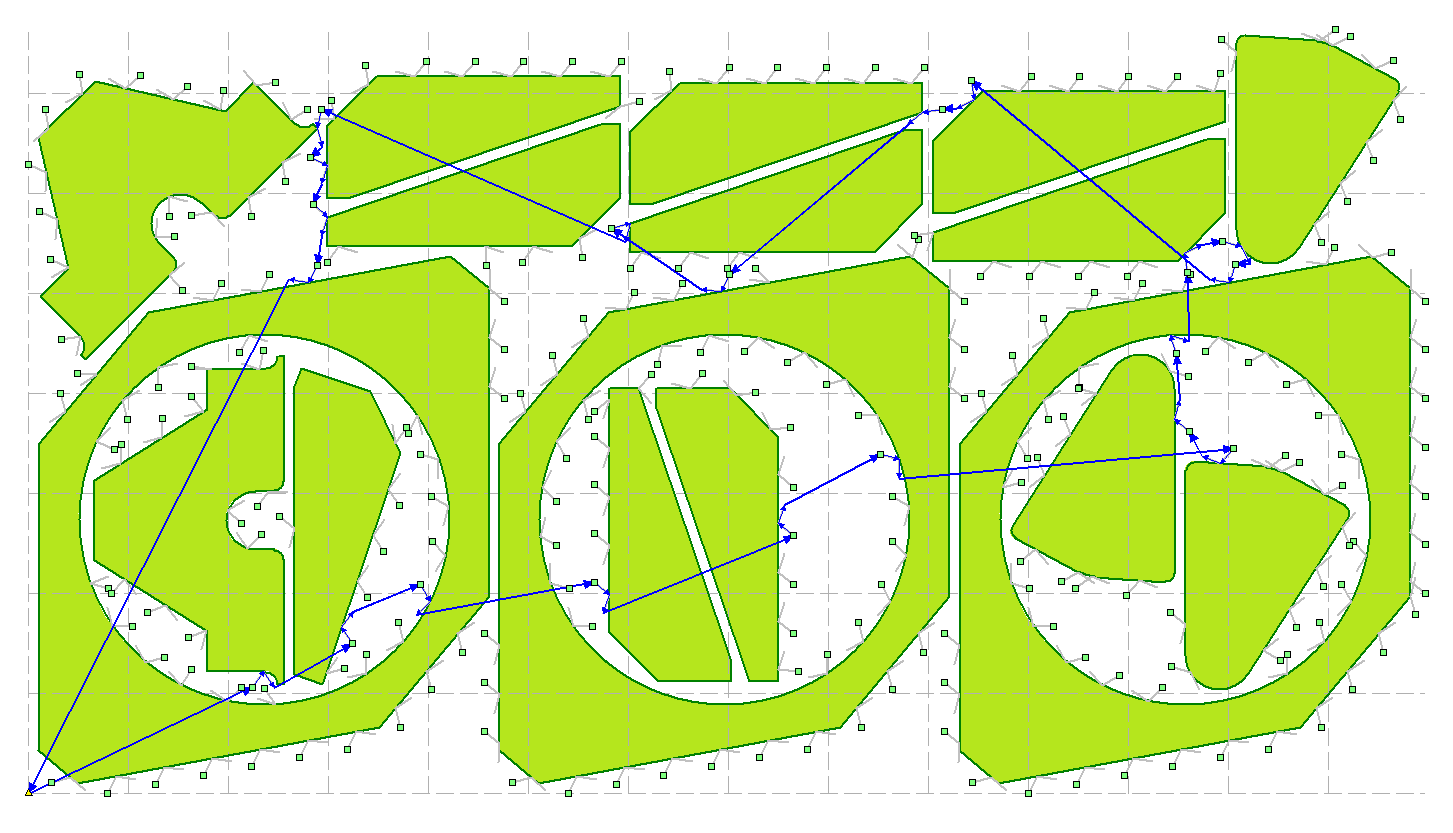
\includegraphics[width=0.9\textwidth]{zones-b.png}
  \caption{Схема оптимального маршрута резки для предыдущего примера}
  \label{zones-b}
  \end{center}
\end{figure}

{\bf Заключительные замечания}

Описанные в данном параграфе практические методы учета
правил жесткости детали и жесткости листа позволяют
имплементировать их в существующие оптимизационные
алгоритмы решения задачи (\ref{problem-statement})
с целевыми функциями \ref{cutting-time} -- \ref{cutting-cost}
и получать рациональные варианты маршрута резки,
уменьшающие геометрические искажения деталей
при термической резке для большинства практических задач.
Вместе с тем, следует отметить,
что описанные способы в некоторых случаях не гарантируют 100 \%
соблюдения технологических требований и
приводят к существенным тепловым деформациям материала.
Помимо этого остается открытым вопрос о разработке
эффективных алгоритмов получения глобальных экстремумов или
близких к ним для решения задач большой размерности с
одновременным учетом всех технологических требований
термической резки, включая динамические ограничения.
Этот вопрос пока еще ждет своего решения.
